\documentclass{article}[18pt]
\ProvidesPackage{format}
%Page setup
\usepackage[utf8]{inputenc}
\usepackage[margin=0.7in]{geometry}
\usepackage{parselines} 
\usepackage[english]{babel}
\usepackage{fancyhdr}
\usepackage{titlesec}
\hyphenpenalty=10000

\pagestyle{fancy}
\fancyhf{}
\rhead{Sam Robbins}
\rfoot{Page \thepage}

%Characters
\usepackage{amsmath}
\usepackage{amssymb}
\usepackage{gensymb}
\newcommand{\R}{\mathbb{R}}

%Diagrams
\usepackage{pgfplots}
\usepackage{graphicx}
\usepackage{tabularx}
\usepackage{relsize}
\pgfplotsset{width=10cm,compat=1.9}
\usepackage{float}

%Length Setting
\titlespacing\section{0pt}{14pt plus 4pt minus 2pt}{0pt plus 2pt minus 2pt}
\newlength\tindent
\setlength{\tindent}{\parindent}
\setlength{\parindent}{0pt}
\renewcommand{\indent}{\hspace*{\tindent}}

%Programming Font
\usepackage{courier}
\usepackage{listings}
\usepackage{pxfonts}

%Lists
\usepackage{enumerate}
\usepackage{enumitem}

% Networks Macro
\usepackage{tikz}


% Commands for files converted using pandoc
\providecommand{\tightlist}{%
	\setlength{\itemsep}{0pt}\setlength{\parskip}{0pt}}
\usepackage{hyperref}

% Get nice commands for floor and ceil
\usepackage{mathtools}
\DeclarePairedDelimiter{\ceil}{\lceil}{\rceil}
\DeclarePairedDelimiter{\floor}{\lfloor}{\rfloor}

% Allow itemize to go up to 20 levels deep (just change the number if you need more you madman)
\usepackage{enumitem}
\setlistdepth{20}
\renewlist{itemize}{itemize}{20}

% initially, use dots for all levels
\setlist[itemize]{label=$\cdot$}

% customize the first 3 levels
\setlist[itemize,1]{label=\textbullet}
\setlist[itemize,2]{label=--}
\setlist[itemize,3]{label=*}

% Definition and Important Stuff
% Important stuff
\usepackage[framemethod=TikZ]{mdframed}

\newcounter{theo}[section]\setcounter{theo}{0}
\renewcommand{\thetheo}{\arabic{section}.\arabic{theo}}
\newenvironment{important}[1][]{%
	\refstepcounter{theo}%
	\ifstrempty{#1}%
	{\mdfsetup{%
			frametitle={%
				\tikz[baseline=(current bounding box.east),outer sep=0pt]
				\node[anchor=east,rectangle,fill=red!50]
				{\strut Important};}}
	}%
	{\mdfsetup{%
			frametitle={%
				\tikz[baseline=(current bounding box.east),outer sep=0pt]
				\node[anchor=east,rectangle,fill=red!50]
				{\strut Important:~#1};}}%
	}%
	\mdfsetup{innertopmargin=10pt,linecolor=red!50,%
		linewidth=2pt,topline=true,%
		frametitleaboveskip=\dimexpr-\ht\strutbox\relax
	}
	\begin{mdframed}[]\relax%
		\centering
		}{\end{mdframed}}



\newcounter{lem}[section]\setcounter{lem}{0}
\renewcommand{\thelem}{\arabic{section}.\arabic{lem}}
\newenvironment{defin}[1][]{%
	\refstepcounter{lem}%
	\ifstrempty{#1}%
	{\mdfsetup{%
			frametitle={%
				\tikz[baseline=(current bounding box.east),outer sep=0pt]
				\node[anchor=east,rectangle,fill=blue!20]
				{\strut Definition};}}
	}%
	{\mdfsetup{%
			frametitle={%
				\tikz[baseline=(current bounding box.east),outer sep=0pt]
				\node[anchor=east,rectangle,fill=blue!20]
				{\strut Definition:~#1};}}%
	}%
	\mdfsetup{innertopmargin=10pt,linecolor=blue!20,%
		linewidth=2pt,topline=true,%
		frametitleaboveskip=\dimexpr-\ht\strutbox\relax
	}
	\begin{mdframed}[]\relax%
		\centering
		}{\end{mdframed}}
\lhead{MCS - Logic and Discrete Structures}


\begin{document}
\begin{center}
\underline{\huge More on propositional logic}
\end{center}
\section{Distribution laws}
Whereas De Morgan’s Laws allow us to simplify formulae with respect to negations we often have “combinations” of disjunctions and conjunctions.\\
\\
The Distributive Law of Disjunction over Conjunction is:\\
$$p\lor (q\land r)\equiv (p\lor q)\land (p\lor r)$$
And the \textbf{Distributive law of conjunction over disjunction is}
$$p\land(q\lor r)\equiv (p\land q)\lor (p\land r)$$
Just as before there are the \textbf{generalised Distributive laws}
$$X\land(Y_1\lor Y_2 \lor ... \lor Y_n)\equiv (X\land Y_1)\lor (X\land Y_2)\lor ... \lor (X\land Y_n)$$
$$X\lor (Y_1\land Y_2 \land ...\land Y_n)\equiv (X\lor Y_1)\land (X\lor Y_2)\land ... \land (X\lor Y_n)$$
Of course we can apply these laws to combinations of formulae and to sub-formulae not just with propositional variables. 
\section{Functional Completeness}
We defined propositional logic using the connectives: $\land \lor \lnot \Rightarrow \Leftrightarrow$, but we could have chosen other connectives\\
\\
We say that a set C of logical connectives is \textbf{functionally complete} if any propositional formula is equivalent to one constructed using only the connectives from C. - This is kind of like Turing complete for logic \\
\\
In fact $\land \lor\lnot$ is functionally complete
\begin{itemize}
\item Let $\varphi$ be a propositional formula involving the variables $p_1,p_2,...,p_n$
\item Build the truth table for $\varphi$ and let f be some truth assignment that evaluates to \textbf{true}
\item Suppose that in this truth assignment f each $p_i$ has the truth value of $v_i$
\item Build a conjunction $\chi_f$ of literals as follows: for each i
\begin{itemize}
\item if $v_i$ is \textbf{true} then include the literal $p_i$ in the conjunction $\chi_f$
\item if $v_i$ is \textbf{false} then include the literal $\lnot p_i$ in the conjunction $\chi_f$
\end{itemize}
\end{itemize}
\subsection{Example}
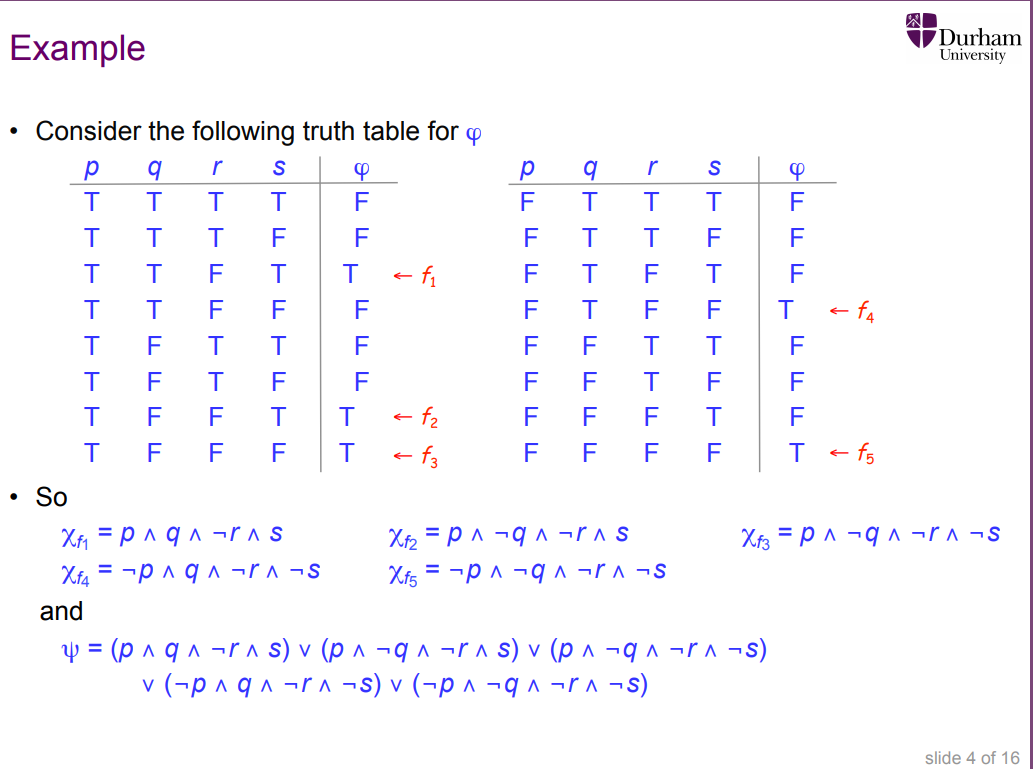
\includegraphics[width=\textwidth]{Fig1.png}
\begin{itemize}
\item $f_1$ can be specified by writing a truth assignment $p\land q\land \lnot r \land s$ 
\item The disjunction can then be written as the lor of all the inputs that make it true, so $\psi={\chi_f}_1\lor...$
\item Only in the case of truth assignment $f_1$ will $\chi_1$ be true and etc for the rest of the fs
\item So this can be used to show that two truth tables are exactly the same, and so that $\land \lor \lnot$ is \textbf{functionally complete}
\end{itemize}
\subsection{More on Functional Completeness}
\begin{itemize}
\item Now let $\psi$ be the disjunction of all those conjunctions $\chi_f$ we have just built. Remember, we only build disjunctions corresponding to the rows of the truth table evaluating to \textbf{true}
\item We claim that $\varphi$ and $\psi$ are logically equivalent
\begin{itemize}
\item Suppose that f is some truth statement making $\varphi$ true, so we have indeed built the conjunction $\chi_f$
\item Key Point: The only truth assignment making the conjunction $\chi_f$ true is the truth assignment f itself
\item In particular the truth assignment f must make $\chi_f$ true
\begin{itemize}
\item For example with regard to the truth assignment f in the example $\chi_f$ is\\ $p_1\land \lnot p_2 \land ... \land \lnot p_n$\\
Which is made \textbf{true} only by the truth assignment f
\end{itemize}
\item Hence, f makes $\psi$ true
\end{itemize}


\item Conversely
\begin{itemize}
\item Suppose that g is some truth assignment making $\psi$ true
\begin{itemize}
\item So at least one conjunct $\chi_f$ say, is made \textbf{true} by g
\end{itemize}
\item But the only truth assignment making $\chi_f$ true is f
\begin{itemize}
\item Hence, f=g
\end{itemize}
\item The reason $\chi_f$ appears as a conjunct is because f makes $\varphi$ true
\begin{itemize}
\item So g=f is a truth assignment making $\varphi$ true
\end{itemize}
\end{itemize}

\item Consequently, for any truth assignment f
\begin{itemize}
\item f satisfies $\varphi$ if, and only if, f satisfies $\psi$
\begin{itemize}
\item That is, $\varphi\equiv\psi$
\end{itemize}
\end{itemize}

\item Our proof yields even more
\begin{itemize}
\item Every formula of propositional logic is equivalent to a formula in \textbf{disjunctive normal form}
\begin{itemize}
\item A disjunction of conjunctions of literals
\end{itemize}
\item Also, every truth table is the truth table of some propositional formula
\end{itemize}
\end{itemize}

\section{Conjunctive normal form}
\begin{itemize}
\item Let $\varphi$ be some formula of propositional logic
\item The formula $\lnot \varphi$ is equivalent to one in disjunctive normal form
\begin{itemize}
\item That is, one of the form\\
$\chi_1\lor\chi_2\lor ... \lor \chi_m$\\
Where each $\chi_i$ is a conjunction of literals
\end{itemize}

\item So, $\varphi$ is equivalent to the formula\\
$\lnot(\chi_1\lor\chi_2\lor ... \lor \chi_m)$\\
Which in turn, by using generalised De Morgan's Laws, is equivalent to\\
$\lnot \chi_1\land \lnot \chi_2\land ... \land \lnot \chi_m$

\item Each $\lnot\chi_i$ is equivalent to a disjunction of literals, by again using generalised De Morgan's Laws

\item Thus
\begin{itemize}
\item Every formula of propositional logic is logically equivalent to a conjunction of disjunctions of literals, i.e., a conjunction of \textbf{clauses}
\begin{itemize}
\item That is, every formula of propositional logic is equivalent to a formula in \textbf{conjunctive normal form}
\end{itemize}
\end{itemize}
\end{itemize}
\section{A spot of practice}
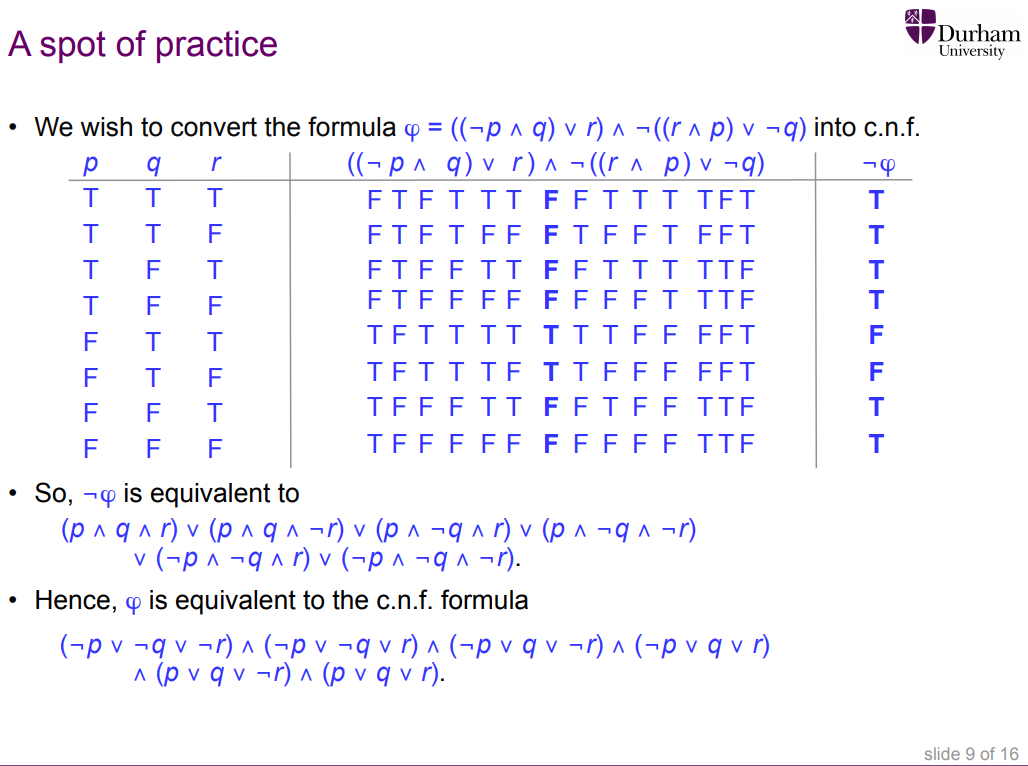
\includegraphics[width=\textwidth]{Fig2.png}

\section{Converting to c.n.f syntactically}
\begin{itemize}
\item We can often establish normal forms "syntactically"
\item Consider the formula\\
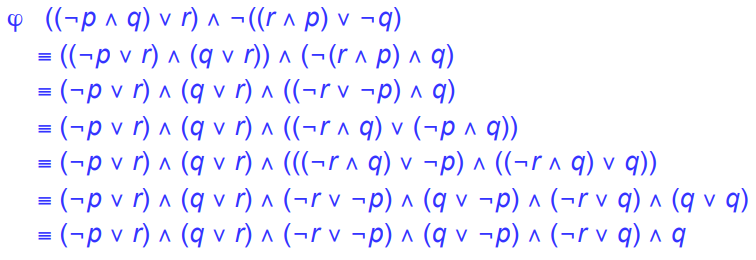
\includegraphics[width=12cm]{Fig3.png}

\item In the "semantic" approach, i.e., using truth tables we are stuck with using exponentially sized truth tables

\item However with the "syntactic" approach, i.e., using known equivalences
\begin{itemize}
\item We can often achieve our aims much more quickly, though this often requires cunning
\end{itemize}
\end{itemize}
\begin{center}
{\huge Non-Examinable from here on}
\end{center}
\section{An application: SAT-solving}
\begin{itemize}
\item The power of propositional logic of quite remarkable as computationally complex problems can be described using logic
\item The aim of SAT-solving is
\begin{itemize}
\item To encode a problem X as a propositional formula $\varphi$ so that
\begin{itemize}
\item A solution to X corresponds to $\varphi$ having a satisfying truth assignment
\end{itemize}
\item To employ algorithms to solve the satisfiability problem (SAT) for $\varphi$ (and so X)
\end{itemize}


\item The SAT problem is to decide if a propositional formula has a satisfying truth assignment. It is extremely hard to solve
\begin{itemize}
\item In fact, it is NP-complete, even if the formula is given in c.n.f, so it takes time exponential in the size of the formula to solve 
\end{itemize} 
\item However, modern day SAT-solvers can give extremely good results
\begin{itemize}
\item Note that all modern day SAT-solvers need their inputs to be in c.n.f
\end{itemize}
\end{itemize}



\end{document}